% This is samplepaper.tex, a sample chapter demonstrating the
% LLNCS macro package for Springer Computer Science proceedings;
% Version 2.20 of 2017/10/04
%
\documentclass[runningheads]{llncs}
%
\usepackage{graphicx}
\usepackage{listings}
\usepackage{microtype}                 % use micro-typography (slightly more compact, better to read)
\PassOptionsToPackage{warn}{textcomp}  % to address font issues with \textrightarrow
\usepackage{textcomp}                  % use better special symbols
\usepackage{mathptmx}                  % use matching math font
\usepackage{times}                     % we use Times as the main font
\usepackage{enumitem}
\renewcommand*\ttdefault{txtt}         % a nicer typewriter font
%\usepackage{cite}                      % needed to automatically sort the references
\usepackage{tabu}                      % only used for the table example
\usepackage{booktabs}                  % only used for the table example
\usepackage{amsmath,amssymb,amsfonts}
\usepackage{subcaption}
\usepackage{framed}
\usepackage{lineno,hyperref}
\newcommand{\fix}[1]{\textcolor{red}{\textbf{\textit{#1}}}}
\newcolumntype{P}[1]{>{\centering\arraybackslash}p{#1}}
\newcolumntype{L}[1]{>{\raggedleft\arraybackslash}p{#1}}
\usepackage[dvipsnames]{xcolor,colortbl}
\newcommand{\mc}[2]{\multicolumn{#1}{c}{#2}}
\definecolor{Gray}{gray}{0.85}
\definecolor{LightCyan}{rgb}{0.88,1,1}
\definecolor{LightRed}{rgb}{1,0.88,1}

\newcolumntype{a}{>{\columncolor{Gray}}c}
\newcolumntype{b}{>{\columncolor{LightCyan}}c}
\newcolumntype{d}{>{\columncolor{LightRed}}c}

\usepackage[subrefformat=parens,labelformat=parens]{subcaption}
\usepackage{multirow}
\usepackage{tikz}
\usepackage{collcell}

\newenvironment{tightEnumerate}{
\begin{enumerate}
        \setlength{\itemsep}{1pt}
        \setlength{\parskip}{0pt}
        \setlength{\parsep}{0pt}
}{\end{enumerate}
}

\newenvironment{tightItemize}{
\begin{itemize}
        \setlength{\itemsep}{1pt}
        \setlength{\parskip}{0pt}
        \setlength{\parsep}{0pt}
}{\end{itemize}
}


\newcommand*{\MinNumberR}{0.0}%
\newcommand*{\MaxNumberR}{20}
\newcommand{\ApplyGradientR}[1]{%
        \pgfmathsetmacro{\PercentColor}{100.0*(#1-\MinNumberR)/(\MaxNumberR-\MinNumberR)}
        \hspace{-0.33em}\colorbox{red!\PercentColor!white}{#1}
}

\newcolumntype{R}{>{\collectcell\ApplyGradientR}c<{\endcollectcell}}



\newcommand*{\MinNumberD}{0}%
\newcommand*{\MaxNumberD}{100}
\newcommand{\ApplyGradientD}[1]{%
        \pgfmathsetmacro{\PercentColor}{100.0*(#1-\MinNumberD)/(\MaxNumberD-\MinNumberD)}
        \hspace{-0.33em}\colorbox{red!\PercentColor!white}{#1}
}







\newcolumntype{D}{>{\collectcell\ApplyGradientD}c<{\endcollectcell}}



\newcommand*{\MinNumberA}{0.0}%
\newcommand*{\MaxNumberA}{0.08}
\newcommand{\ApplyGradientA}[1]{%
        \pgfmathsetmacro{\PercentColor}{100.0*(#1-\MinNumberA)/(\MaxNumberA-\MinNumberA)}
        \hspace{-0.2em}\vspace{-0.05em}\colorbox{orange!\PercentColor!white}{#1}
}

\newcolumntype{A}{>{\collectcell\ApplyGradientA}c<{\endcollectcell}}


\newcommand*{\MinNumberB}{0.0}%
\newcommand*{\MaxNumberB}{10.0}
\newcommand{\ApplyGradientB}[1]{%
        \pgfmathsetmacro{\PercentColor}{100.0*(#1-\MinNumberB)/(\MaxNumberB-\MinNumberB)}
        \hspace{-0.2em}\colorbox{orange!\PercentColor!white}{#1}
}

\newcolumntype{B}{>{\collectcell\ApplyGradientB}c<{\endcollectcell}}


\newcommand*{\MinNumberC}{0.0}%
\newcommand*{\MaxNumberC}{0.44}
\newcommand{\ApplyGradientC}[1]{%
        \pgfmathsetmacro{\PercentColor}{100.0*(#1-\MinNumberC)/(\MaxNumberC-\MinNumberC)}
        \hspace{-0.2em}\colorbox{orange!\PercentColor!white}{#1}
}

\newcolumntype{C}{>{\collectcell\ApplyGradientC}c<{\endcollectcell}}


\newcommand*{\MinNumberN}{0.0}%
\newcommand*{\MaxNumberN}{0.75}
\newcommand{\ApplyGradientN}[1]{%
        \pgfmathsetmacro{\PercentColor}{100.0*(#1-\MinNumberN)/(\MaxNumberN-\MinNumberN)}
        \hspace{-0.33em}\colorbox{red!\PercentColor!white}{#1}
}

\newcolumntype{N}{>{\collectcell\ApplyGradientN}c<{\endcollectcell}}

\usepackage{epstopdf}
\epstopdfsetup{outdir=./}
% Used for displaying a sample figure. If possible, figure files should
% be included in EPS format.
%
% If you use the hyperref package, please uncomment the following line
% to display URLs in blue roman font according to Springer's eBook style:
% \renewcommand\UrlFont{\color{blue}\rmfamily}

\begin{document}
%
\title{Investigating In Situ Reduction \\via Lagrangian Representations\\ for Cosmology and Seismology Applications}
%
\titlerunning{Lagrangian Representations for Cosmology and Seismology Applications}
% If the paper title is too long for the running head, you can set
% an abbreviated paper title here
%
%\author{Sudhanshu Sane\inst{1}\orcidID{0000-1111-2222-3333} \and Hank Childs\inst{2}\orcidID{1111-2222-3333-4444}}
%
\authorrunning{S. Sane et al.}
% First names are abbreviated in the running head.
% If there are more than two authors, 'et al.' is used.
%
\institute{SCI Institute at University of Utah, USA \and University of Oregon, USA}
%
\author{Sudhanshu Sane\inst{1} \and Chris R. Johnson\inst{1} \and Hank Childs\inst{2}}
\institute{SCI Institute at University of Utah, USA \and University of Oregon, USA}
\maketitle              % typeset the header of the contribution
%
\begin{abstract}
Although many types of computational simulations produce time-varying vector fields,
subsequent analysis is often limited to single time slices due to excessive costs.
%
Fortunately, a new approach using a Lagrangian representation can
enable time-varying vector field analysis while mitigating these costs.
%
With this approach, a Lagrangian representation is calculated while the simulation code is running, and the result is explored after the simulation.
%
Importantly,
 the effectiveness of this approach varies based on the nature of the vector field,
requiring in-depth investigation for each application area.
%
With this study, we evaluate the effectiveness for previously unexplored cosmology and seismology
applications. %, which have previously been unexplored.
%
We do this by considering encumbrance (on the simulation) and accuracy (of the reconstructed result).
%
To inform encumbrance, we
integrated in situ infrastructure with two simulation codes,
and evaluated on representative HPC environments,
performing Lagrangian in situ reduction using GPUs as well as CPUs.
%
To inform accuracy, our study conducted a statistical analysis across a range of spatiotemporal configurations as well as a qualitative evaluation.
%
In all, we demonstrate effectiveness for both cosmology and seismology --- time-varying vector fields from these domains can be reduced to less than 1\% of the total data via Lagrangian representations, while maintaining accurate reconstruction and requiring under 10\% of total execution time in over 80\% of our experiments.
\keywords{Lagrangian analysis \and in situ processing \and vector data}
\end{abstract}
%

\section{Introduction}
\label{sec:introduction}
High-performance computing resources play a key role in advancing computational science by enabling modeling of scientific phenomena at high spatiotemporal resolutions.
%
%Although HPC enables modeling of scientific phenomena at high spatiotemporal resolutions, the total data generated is prohibitively large.
%
A challenge with regard to studying the output of a simulation is the prohibitively large size of the total data generated.
%
Compromise in the form of storing a subset of the data can impact the extent and accuracy of subsequent post hoc exploratory analysis and visualization.
%
In particular, for accurate time-varying vector field analysis and visualization, access to the full spatiotemporal resolution is required.
%
Since storing the entire simulation output is expensive, scientists resort to temporal subsampling or lossy compression, and often limit analysis to individual time slices.
%
An emerging paradigm to address large data challenges is the use of in situ processing to perform runtime analysis/visualization or data reduction to support exploratory post hoc analysis.
%
%

%
Lagrangian analysis is a powerful tool to study time-varying vector fields and is widely employed for ocean modeling applications~\cite{VANSEBILLE201849}.
%
The notion of calculating a Lagrangian representation or \textit{flow map}, i.e., sets of particle trajectories, ``online'' (in situ) for ``offline'' (post hoc) exploration was first proposed by Vries et al.~\cite{vries2001calculating} for an ocean modeling simulation.
%
Figure~\ref{fig:sample} illustrates the approach.
%
More recently, multiple works have advanced Lagrangian research along axes such as strategies for in situ extraction of reduced Lagrangian representations~\cite{agranovsky2014improved}\cite{rapp2019void}\cite{sane2020scalable}, post hoc reconstruction~\cite{chandler2015interpolation}\cite{sane2019interpolation}\cite{Jakob20}, and theoretical error analysis~\cite{bujack2015lagrangian}\cite{chandler2016analysis}\cite{hummel2016error}.
%

An open challenge for time-varying vector field exploration is predicting the uncertainty and variability in accuracy for different analysis techniques.
%
Although the effectiveness of Lagrangian representations for any possible time-varying vector field that can be produced by a scientific simulation remains an open question, prior theoretical demonstration of Lagrangian techniques~\cite{agranovsky2014improved}\cite{chandler2015interpolation}\cite{bujack2015lagrangian}\cite{chandler2016analysis}\cite{hummel2016error}\cite{sane2018revisiting}\cite{sane2019interpolation}\cite{rapp2019void}\cite{Jakob20} on analytical, SPH, climate and ocean modeling data, and practical application in ocean activity analysis~\cite{siegfried2019tropical}, has provided encouraging results.
%
Using Lagrangian representations, the quality of post hoc reconstruction depends on the vector field itself, as well as configuration specifics such as sampling strategy and frequency of storage.
%
Thus, to investigate the potential benefits of Lagrangian representations for a broader range of applications and to gauge its viability in practice, we leverage the recent developments of runtime in situ infrastructure that enable the straightforward extraction via APIs to study Lagrangian representations for cosmology and seisomology applications.

\begin{figure}[!t]
\centering
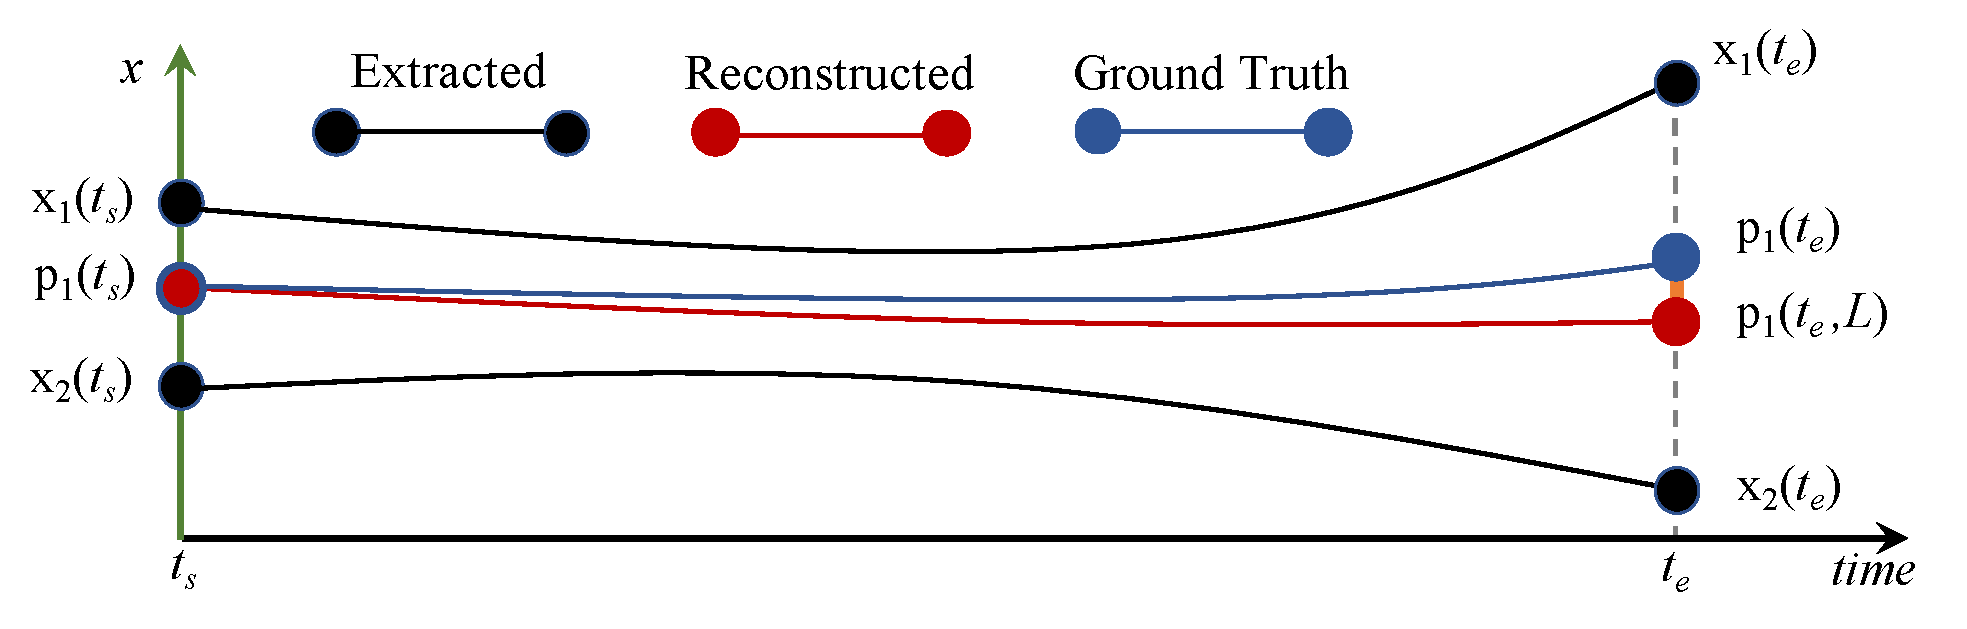
\includegraphics[width=0.85\linewidth]{sample.pdf}
\vspace{-3mm}
\caption{Notional space-time visualization of Lagrangian representations for a time-varying 1D flow. The black trajectories are computed in situ and encode the behavior of the vector field between start time \textit{t$_{s}$} and end time \textit{t$_{e}$}. In a post hoc setting, a Lagrangian-based advection scheme \textit{L}, i.e., a technique to interpolate the extracted data, is used to calculate the trajectory of a new particle p$_{1}$ . The red trajectory is the trajectory reconstructed post hoc and the blue trajectory is the ground truth. The end location of the red trajectory deviates by a margin of error from the ground truth.}
%The quality of reconstruction often depends on the nature of the time-varying vector field.}
\vspace{-8mm}
\label{fig:sample}
\end{figure}

In this paper, our unique contribution is an investigation of Lagrangian representations to encode self-gravitating gas dynamics of a cosmology simulation and seismic wave propagation of a seisomology simulation.
%
We measure the effectiveness of the technique by considering in situ encumbrance and post hoc accuracy.
%
For both applications, our experiments show that Lagrangian representations offer high data reduction, in many cases requiring less than 1\% storage of the complete time-varying vector fields, for a small loss of accuracy.
%
Further, our study shows Lagrangian representations are viable to compute in representative HPC environments, requiring under 10\% of total execution time for data analysis and visualization in the majority of configurations tested.

\vspace{-2mm}
\section{Background and Related Work}
\label{sec:related}
\vspace{-1mm}
\subsection{Frames of Reference}
\setlength{\belowdisplayskip}{3pt} \setlength{\belowdisplayshortskip}{3pt}
\setlength{\abovedisplayskip}{3pt} \setlength{\abovedisplayshortskip}{3pt}
%
In fluid dynamics, there are two frames of reference to observe fluid motion: Eulerian and Lagrangian.
%
With the Eulerian frame of reference, the observer is in a fixed position.
%
With the Lagrangian frame of reference, the observer is attached to a fluid parcel and is moving through space and time.

%
Storage of a flow field in an Eulerian representation is typically done by means of its velocity field.
%
A velocity field $v$ is a time-dependent vector field that maps each point $x\in \mathbb R^d$ in space to the velocity of the flow field for a given time $t\in \mathbb R$
%
\begin{eqnarray}
{v} : \mathbb R^d \times \mathbb R \to \mathbb R^d,\; x,t \mapsto v(x,t)
\end{eqnarray}

%
In a practical setting, a flow field at a specific time/cycle is defined as vector data on a fixed, discrete mesh.
%
Time-varying flow is represented as a collection of such data over a variety times/cycles.


Storage of a flow field in a Lagrangian representation is done by means of its flow map $F_{t_0}^{t}$.
%
The flow map is comprised of the starting positions of massless particles $x_0$ at time $t_0$ and their respective trajectories that are interpolated using the time-dependent vector field.
%
Mathematically, a flow map is defined as the mapping
\begin{eqnarray}
F_{t_0}^{t}(x_0):\mathbb R \times \mathbb R \times \mathbb R^d \to \mathbb R^d,\; t \times t_0 \times x_0 \mapsto F_{t_0}^{t}(x_0) = x(t)
\end{eqnarray}
%
of initial values $x_0$ to the solutions of the ordinary differential equation
%
\begin{eqnarray}
\frac{d}{dt}x(t) = v(x(t),t)
\end{eqnarray}

In a practical setting, the flow map is represented as sets of particle trajectories calculated in the time interval $[t_0,t]\subset \mathbb R$.
%
The stored information, encoded in the form of known particle trajectories (i.e., a Lagrangian representation), encodes the behavior of the time-dependent vector field over an interval of time.
%
\renewcommand{\baselinestretch}{1}

\vspace{-1mm}
\subsection{Lagrangian Analysis}
Within the vector field analysis and visualization community, Lagrangian methods have been increasingly researched in the past decade.
%
In this paper, we focus on the use of Lagrangian methods to store time-varying vector fields in situ and enable subsequent post hoc analysis.
%
%fueled by temporal sparsity of data, i.e., simulations store data less frequently to avoid high storage costs.
%
In sparse temporal settings, Lagrangian representations are expected to perform better than their Eulerian counterparts.
%
The key intuition behind this expectation is that Lagrangian representations capture the behavior of the flow field over an interval of time, as opposed to the state at a single time slice.
%
However, in addition to the frequency of temporal sampling, the nature of the vector field and spatial sampling resolution impacts the quality of reconstruction.
%

Agranovsky et al.~\cite{agranovsky2014improved} conducted the seminal work to evaluate the efficacy of reduced Lagrangian representations.
%
To maintain domain coverage, the study proposed the use of uniform spatial sampling to extract sets of temporally non-overlapping basis trajectories.
%
Sane et al.~\cite{sane2018revisiting} studied performance across a range of spatiotemporal configurations when operating using a fixed storage budget.
%
The experiments in these works were conducted in a theoretical in situ setting, i.e., files were loaded from disk. %rather than integration with a simulation.
%
Most recently, Jakob et al.~\cite{Jakob20} trained a DNN to upsample FTLE visualizations derived from reduced Lagrangian representations.
%
To generate training data, they first computed Lagrangian representations of a 2D flow field using a tightly-coupled integration with an open-source CFD solver on HPC resources and reported computation costs.
%
However, the grid size of $4\times4$ per rank used in the study is not representative of real-world applications.
%
Thus, the current literature lacks in situ encumbrance measurements in representative settings.
%

Lagrangian representations of a time-varying vector field can be extracted by adopting various strategies.
%
Sane et al.~\cite{sane2019interpolation} explored computing trajectories of variable duration and placement.
%and consequently proposed a post hoc interpolation scheme to reduce reconstruction error by evaluating neighborhoods across interpolations.
%
Rapp et al.~\cite{rapp2019void} applied their void-and-cluster sampling technique to identify a representative set of scattered samples.
%
Although these strategies improved accuracy, they increased computation costs and are presently limited to single node settings.
%
To address scalability challenges of extracting a Lagrangian representation in distributed memory, Sane et al.~\cite{sane2020scalable} explored an accuracy-performance tradeoff and demonstrated the use of a communication-free model that stored only trajectories that remain within the rank domain during the interval of computation.
%

Prior works have presented research pertaining to post hoc reconstruction using Lagrangian-based interpolation schemes.
%
Hlawatsch et al.~\cite{hlawatsch2011hierarchical} proposed a hierarchical reconstruction scheme that can improve accuracy, but relies on access to data across multiple time intervals.
%
Chandler et al.~\cite{chandler2015interpolation} proposed a modified k-d tree as a search structure for Lagrangian data extracted from an SPH simulation.
%
Further, Chandler et al.~\cite{chandler2016analysis} identified correlations between Lagrangian-based interpolation error and divergence in the flow field.
%
Bujack et al.~\cite{bujack2015lagrangian} evaluated the use of parameter curves to fit interpolated pathline points to improve the aesthetic of trajectories calculated using Lagrangian data.
%
Lastly, Hummel et al.~\cite{hummel2016error} provided theoretical error bounds for error propagation that can occur when calculating trajectories using Lagrangian representations.
%

\vspace{-1mm}
\subsection{Time-Varying Vector Field Reduction}
%
Although Eulerian representations have been shown to be susceptible to temporal sparsity~\cite{costa2004lagrangian}\cite{Qin2014}\cite{agranovsky2014improved}\cite{sane2018revisiting}, temporal subsampling remains the widely used solution to limit data storage.
%
Our study adds to this body of work by using temporal subsampling for comparison.
%
Multiple works have proposed single time step vector field reduction strategies while maintaining an Eulerian representation~\cite{lodha2003topology}\cite{theisel2003combining}\cite{tong2012salient}.
%
Although these techniques could be used to reduce and store data more frequently, they do not inherently address the challenge of increasing temporal sparsity.
%

In a recent large-scale tornadic supercell thunderstorm study~\cite{atmos10100578}, Leigh Orf modified the I/O code to use a hierarchical data format and lossy floating-point compression via ZFP~\cite{lindstrom2006fast}.
%
ZFP provides dynamic accuracy control by allowing the user to specify a maximum amount of deviation.
%
Orf stated that although ZFP is effective for scalar fields that do not require differentiation during post hoc analysis, only a very small value of deviation can be chosen for each component of velocity to maintain accurate time-varying vector field reconstruction.
%
Thus, ZFP allowed a limited amount of compression to vector field data without introducing significant uncertainty to post hoc analysis.
%
The technique provided an average reduction of 30\% of total uncompressed vector field data, with regions of high gradient resulting in less compression.
%
Overall, Orf referred to the use of lossy compression as unfortunate but necessary.

\vspace{-2mm}
\section{In Situ Reduction via Lagrangian Representations}
\label{sec:method}
\begin{figure}[!t]
\centering
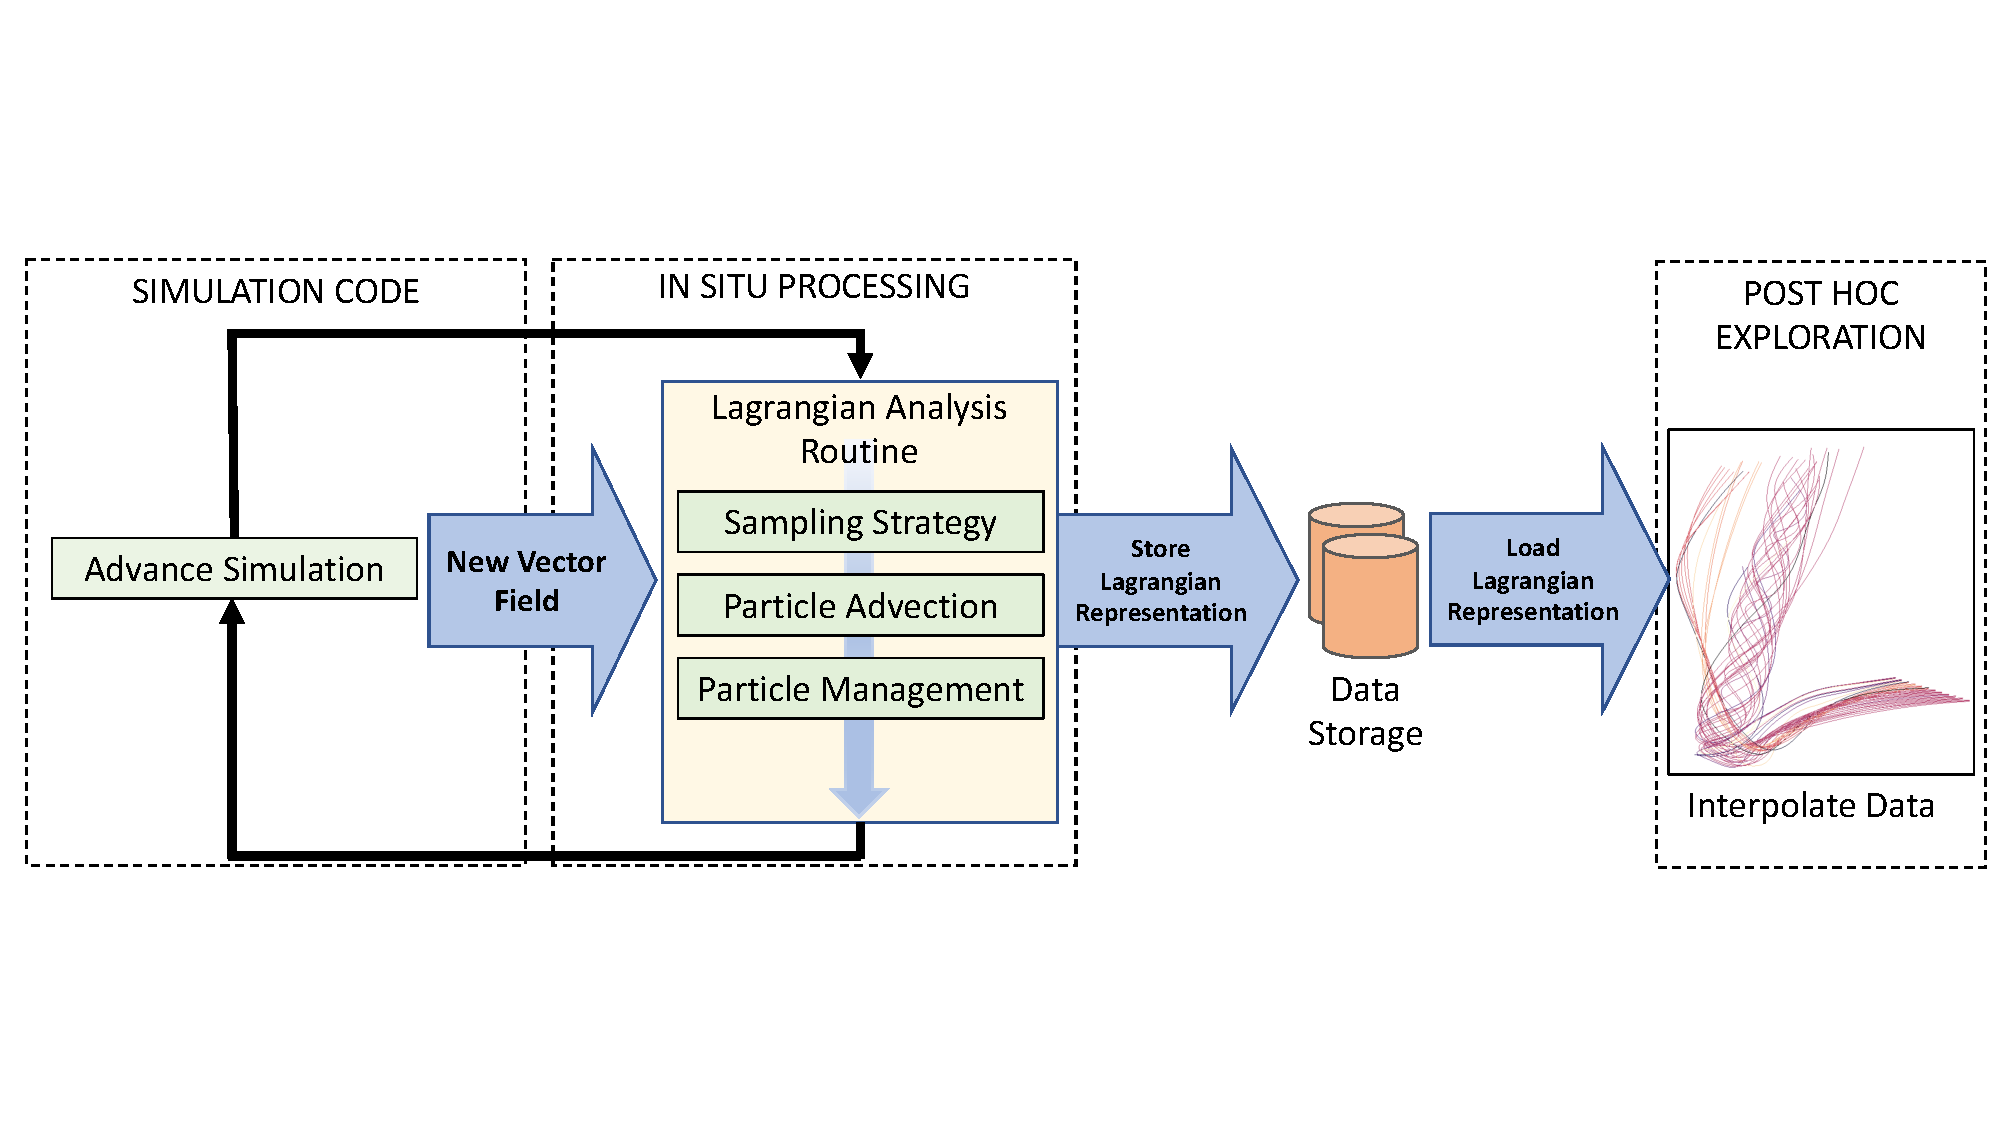
\includegraphics[width=0.9\linewidth,trim={0cm 4.3cm 0cm 4.3cm}, clip ]{Schematic.pdf}
\vspace{-2mm}
\caption{Schematic of the Lagrangian in situ reduction and post hoc exploration workflow.} %the simulation code with in situ processing integrated, data storage, and post hoc analysis.}
\vspace{-5mm}
\label{fig:schematic}
\end{figure}

This section describes the instantiation we consider for our study.
%
Figure~\ref{fig:schematic} shows a high-level description of the Lagrangian in situ reduction post hoc exploration (L-ISR-PHE) workflow.
%
%There are many possible strategies for accomplishing the components within this workflow.
%
For our study, we focused on the current best practices in this space.
%
To describe our instantiation, the remainder of this section is divided based on the two phases: in situ reduction and post hoc exploration.
%

\noindent\textbf{In Situ Reduction}
%
Both simulations we considered partitioned space amongst ranks,
with each rank owning one portion of the vector field.
Our in situ routines followed this pattern, with an
instance of our Lagrangian analysis
routine executing for each rank, accessing its portion
of the vector field.
%
Further, for both simulations we were interested in capturing time-varying vector field behavior across the entire domain.
%
Thus, for our in situ data reduction strategy, we prioritized domain coverage.
%
Similar to Agranovsky et al.~\cite{agranovsky2014improved}, we used uniform spatial sampling and a predetermined interval to store/reset particles.
%
Thus, we computed sets of temporally non-overlapping basis trajectories over the duration of the simulation.
%
Each set of basis trajectories encodes the behavior of the time-varying vector field over a specific interval of time.
%
Our particle termination followed the local Lagrangian flow map model from Sane et al.~\cite{sane2020scalable}, where particles are terminated once they reach the end of the interval or exit the block.
%
Our implementation had two main knobs that control the total data storage and quality of reconstruction: number of basis trajectories, i.e., spatial sampling resolution, and frequency of storing information to disk, i.e., storage interval.
%
The effect of these settings varies depending on the underlying vector field.
%

We used the Ascent~\cite{Larsen2017Alpine} in situ infrastructure and VTK-m~\cite{moreland2016vtk} library to implement L-ISR.
%
The Ascent API can be used to perform tightly-coupled integration with an application code and access various in situ analytics capabilities.
%%
The VTK-m Lagrangian filter on each rank operated independently and maintained its own list of particles.
%
We used the existing particle advection infrastructure available in VTK-m~\cite{pugmire2018performance}.
%
RK4 particle advection is implemented using VTK-m worklets (kernels) that offer performance portability by utilizing the underlying hardware accelerators.
%
In our implementation, each Lagrangian filter stored the displacement of each particle (three double), as well as its validity (one Boolean), i.e., whether the particle remained within the domain during the interval of calculation.
%
Overall, computing a Lagrangian representation increased the runtime memory cost on the simulation by approximately by four one-dimensional simulation ``fields''.
%
Simulations often have tens to hundreds of fields defined on the simulation grid, and thus, this cost would likely be acceptable for most simulations.
%
%In more complicated frameworks, it is possible to associate additional information (for example, ID, age, start location, previous locations, etc.) with each particle at the cost of higher runtime memory usage and data storage.
%

To compute a Lagrangian representation, the simulation invoked Ascent after every cycle it advanced.
%
Ascent accessed the simulation vector field data and consequently invoked the Lagrangian filter.
%
The Lagrangian filter used the vector field to advance particles, and triggered the storage of trajectories at the end of an interval.
%
%In our implementation, following previous work~\cite{agranovsky2014improved}\cite{sane2018revisiting}\cite{sane2020scalable}, a trajectory in the Lagrangian representation is stored using a start and end location.
%
For integration, all the steps involved --- creating an instance of Ascent, specifying parameters, and invoking the VTK-m Lagrangian filter --- required only 23 lines of code (C++). % and less is a JSON input file was used.
%
%The code sample in Listing~\ref{lst:code} shows these steps.
%

\noindent\textbf{Post Hoc Exploration}
For post hoc analysis, new particle trajectories are computed to explore the time-varying vector field. %by interpolating basis trajectories that were extracted in situ.
%
To construct new particle trajectories, we first identified which basis trajectories to follow and then performed interpolation.
%
Based on the study of accuracy of various Lagrangian-based advection schemes in~\cite{agranovsky2015subsampling}, our study employed a Delaunay triangulation to identify the neighborhood of valid basis trajectories and second-order barycentric coordinates for interpolation.
%
We used the CGAL~\cite{fabri2011cgal} library to construct and search the Delaunay triangulation.
%
After constructing new pathlines or deriving new scalar fields from the basis trajectories, we used VisIt~\cite{childs2012visit} to generate visualizations.

\vspace{-2mm}
\section{Study Overview}
\label{sec:study}
This section provides an overview of our study. It is organized as follows: runtime environment~(\ref{sec:runtime}), simulation codes~(\ref{sec:simulations}), experiments~(\ref{sec:experiments}), and evaluation metrics~(\ref{sec:metrics}). %, and runtime environment~(\ref{sec:runtime}).

\vspace{-3mm}
\subsection{Runtime Environment}
\label{sec:runtime}
Our study used the Summit supercomputer at ORNL.
%
A Summit compute node has two IBM Power9 CPUs, each with 21 cores running at 3.8 GHz and 512 GBytes of DDR4 memory.
%
Nodes on Summit also have enhanced on-chip acceleration with each CPU connected via NVLink to 3 GPUs, for a total of 6 GPUs per node.
%
Each GPU is an NVIDIA Tesla V100 with 5120 CUDA cores, 6.1 TeraFLOPS of double precision performance, and 16 GBytes of HBM2 memory.
%
Lastly, it has a Mellanox EDR 100G InfiniBand, Non-blocking Fat Tree as its interconnect topology.

\vspace{-3mm}
\subsection{Simulation Codes}
\label{sec:simulations}

\textbf{Nyx:} In this cosmological simulation~\cite{almgren2013nyx}, baryonic matter is evolved by solving the equations of self-gravitating gas dynamics.
%
We derived the velocity field using the fields of momentum and density of the baryonic gas.
%
The simulation involves particles gravitating toward high-density regions to form multiple clusters across the domain.
%
The distribution of high-density clusters and their formation is of interest to scientists.
%
To study the distribution, scientists currently perform statistical analysis of gas particle density at a single time slice.
%
We investigated the potential of reduced Lagrangian representation to accurately visualize the particle evolution and the distribution of high-density clusters using pathlines.
%
%
The Nyx simulation we built executed as a single rank using two CPUs on a single Summit compute node.
%

\noindent\textbf{SW4:} In this seismology simulation~\cite{petersson2015wave}, seismic wave propagation is studied using a fourth-order method.
%
The application simulates waves radiating from the epicenter through viscoelastic media.
%
%
We used the 3D time-varying displacement vector defined at each grid point as input.
%
We investigated how accurately we can derive and visualize the field encoding displacement over time in two regions: at the epicenter and away from the epicenter.
%
The SW4 simulation we built executed using six ranks per compute node on Summit. Each rank was allocated a GPU for execution.
%

%
\vspace{-3mm}
\subsection{Experiments}
\label{sec:experiments}

For each application in this study, we organized our experiments to inform in situ encumbrance and post hoc accuracy.
%
We considered four evaluation criteria (EC).
%
To inform in situ encumbrance,  we measured the execution time (EC1) and runtime memory usage (EC2) for in situ processing.
%
To inform post hoc accuracy, we measured the size of data artifacts (EC3) and the reconstruction quality of time-varying vector field data (EC4).
%
Next, we identified four factors that when varied produce the workloads we want to evaluate for our study:
\begin{tightItemize}
\item\textbf{Number of particles:} the spatial sampling resolution denoted using \textbf{1:X}, where X is the reduction factor. For example, a 1:8 configuration states that one basis particle is used for every 8 grid points ($\approx$12.5\% of the original data size).
\item\textbf{Storage interval:} the number of cycles between saves and denoted by \textbf{I}.
\item\textbf{Grid size:} the spatial resolution of the mesh.
\item\textbf{Concurrency:} the scale of the execution and underlying parallelization hardware.
\end{tightItemize}
%
Rather than consider a complete cross-product of options for every workload factor, we sampled the space of possible options.
%
Our goal was to provide coverage and allow us to see the impact of certain workload factors, all while staying within our compute budget.
%
For Nyx, we ran 18 experiments, with 6 informing in situ encumbrance (varying \textbf{1:X}, grid size) and 12 informing post hoc accuracy (varying \textbf{1:X}, \textbf{I}).
%
For SW4, we ran 11 experiments, with 7 informing in situ encumbrance (varying \textbf{1:X}, grid size, concurrency) and 4 informing post hoc accuracy (varying \textbf{1:X}).
%
The specific options selected are presented along with the results in Section~\ref{sec:results}.

\vspace{-3mm}
\subsection{Evaluation Metrics}
\label{sec:metrics}
We selected our evaluation metrics based on the evaluation criteria listed in Section~\ref{sec:experiments}.
%

For EC1, we measured the average cost of invoking the Lagrangian VTK-m filter through Ascent every cycle, \textbf{Step}, in seconds. Additionally, we presented the percentage of simulation time spent on data analysis and visualization, or \textbf{DAV\%}.
%
We used \textbf{Sim$_{cycle}$} to denote the average time required for a single simulation cycle in seconds.

For EC2, we measured \textbf{InSituMem}, the runtime memory cost incurred by every compute node to maintain the state (current position) of particles at runtime in Bytes.
%

For EC3, we measured the total data storage (\textbf{DS}) required on the file system and report it in Bytes stored.
%
In addition to I/O being infrequently performed, we observed that for the scale of study we conducted, Summit provided fast write times.
%
In comparison to performing in situ processing every cycle, we found the I/O write cost to be negligible. %at the scale we test.

For EC4, we considered both a statistical and qualitative analysis.
%
For Nyx, we derived pathlines from the basis trajectories and measured the reconstruction error by calculating the average Euclidean distance of interpolated points from the ground truth~(precomputed using the complete simulation data) for each trajectory.
%
We visualized the distribution of pathline reconstruction error for every configuration using violin plots, and for a subset of configurations, the pathline clustering directly.
%
For SW4, we derived a field encoding magnitude of displacement over time from the basis trajectories.
%
In this case, we visualized and compared the derived field to the ground truth time-varying displacement field using violin plots and isosurfaces.

\vspace{-2mm}
\section{Results}
\label{sec:results}
Our results are organized as follows.
%
Sections~\ref{sec:nyx} and~\ref{sec:sw4} present findings from our study investigating reduced Lagrangian representations for cosmology and seismology applications, respectively.
%
%Section~\ref{sec:cloverleaf3d} contains results from our benchmarking study.
%
Tables~\ref{table:nyx_encumbrance} and~\ref{table:sw4_encumbrance} provide information pertaining to in situ encumbrance experiments, such as concurrency information, spatial dimensions, Sim$_{cycle}$, number of particles per compute node, \textbf{InSituMem} per compute node, \textbf{Step}, and \textbf{DAV\%}, for each application.
%
Figure~\ref{fig:insitucost} shows the execution time per cycle for all the in situ encumbrance experiments. %from both applications.
%
\begin{figure}[!t]
\centering
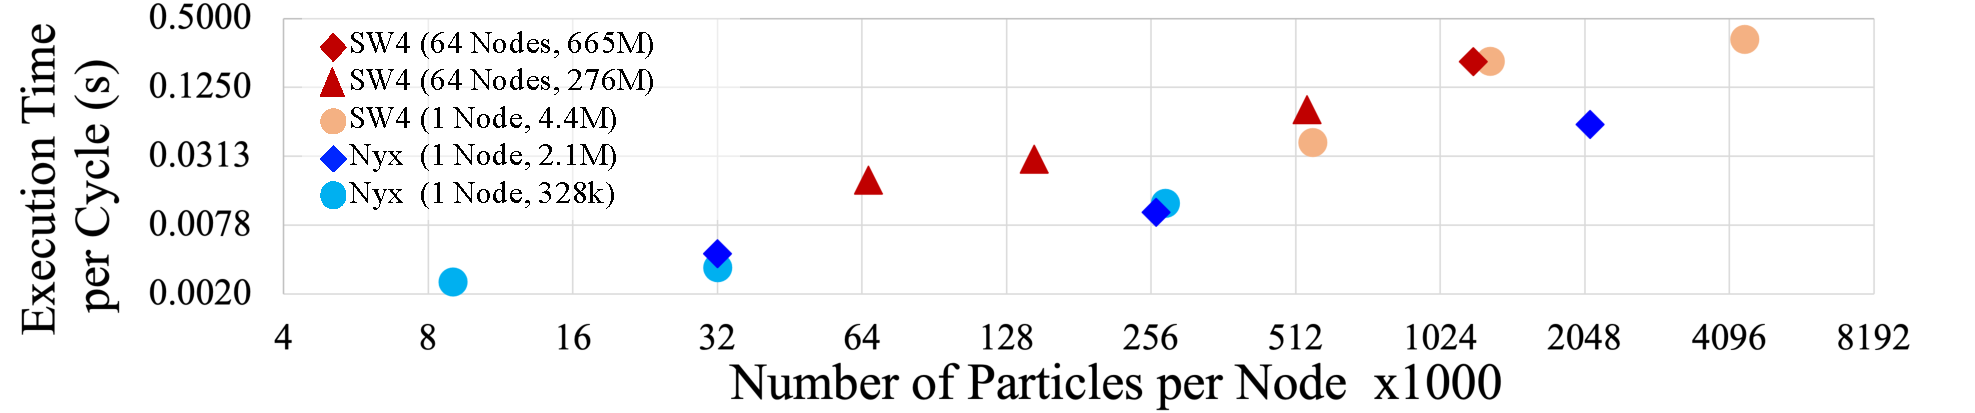
\includegraphics[width=\linewidth]{InSituCost_Stretch2.pdf}
\vspace{-5mm}
\caption{Lagrangian in situ reduction cost per cycle for all in situ encumbrance experiments. The SW4 simulation executes with six ranks (each allocated one GPU) sharing memory on every node. The Nyx simulation executes on a single rank using all the cores of two CPUs on a single node. The legend includes concurrency and number of simulation grid points in parenthesis and both axes use logarithmic scales.}
\vspace{-5mm}
\label{fig:insitucost}
\end{figure}
%
Figures~\ref{fig:nyx_violinplot},~\ref{fig:nyx_figure},~\ref{fig:sw4_violinplot}, and ~\ref{fig:sw4_figure} show the results of our post hoc accuracy evaluation.
%
For each application, the figures are annotated with configuration specifics such as the \textbf{DS}, \textbf{1:X}, and \textbf{I}.
%
Further, Lagrangian and Eulerian tests are distinguished explicitly in the captions or are labeled L$T$ and E$T$, respectively, where $T$ is the test number.
%

\vspace{-3mm}
\subsection{Nyx Cosmology Simulation}
\label{sec:nyx}
\noindent\textbf{In Situ Encumbrance}
Using all the cores of two CPUs on a single compute node, we used OpenMP to parallelize the Nyx simulation and Lagrangian VTK-m filter.
%
We tested two options for grid size - $69^{3}$ and $129^{3}$ - on a single rank, and three particle advection workloads (1:1, 1:8, 1:27) each.
%
In a single compute node hour, the simulation performed approximately 300 and 38 cycles when using $69^{3}$ and $129^{3}$ grid sizes, respectively.
%
%In a single compute node hour, the simulation performs approximately 300 cycles for the $69^{3}$ resolution and approximately 38 cycles for the $129^{3}$ resolution.
%
An 8X increase in grid size resulted in a proportional increase in Sim$_{cycle}$ but only a small increase in particle advection costs for the same number of particles.
%
In practice, we would expect a single rank to operate on between $32^{3}$ to $256^{3}$ grid points, and thus our workloads provided a representative estimate of \textbf{DAV\%}.
%
%For example, sampling a $256^{3}$ using a 1:8 reduction involves computing 2.1M basis trajectories.

An encouraging finding was the low in situ encumbrance when performing L-ISR on the CPUs.
%
Depending on the setup of various simulations and the form of integration for in situ processing, future work can consider offloading L-ISR computation to CPUs.
%
Overall, considering the longer Sim$_{cycle}$ times for the Nyx simulation, and parallel compution coupled with low memory latency when using CPUs, the highest in situ encumbrance to extract a Lagrangian represenation was 0.1\% of the simulation time or under 0.06s to compute 2.1M basis trajectories per cycle.\\
\begingroup
\setlength{\tabcolsep}{-2pt}
\begin{table*}[!t]
\centering
\begin{tabular}{|P{1.1cm}|P{1.1cm}|P{2.7cm}|P{1.3cm}|P{1.5cm}|P{1.9cm}|P{1.7cm}|P{1.7cm}|}
\hline
Nodes & Ranks & Dimensions & \textbf{Sim$_{cycle}$} & Particles & \textbf{InSituMem} & \textbf{Step} & \textbf{DAV\%} \\
\hline
\cline{1-8}
\multirow{6}{*}{1} & \multirow{6}{*}{1} & \multirow{3}{*}{$65\times65\times65$} & \multirow{3}{*}{10.9s} & 9k & 0.2MB & 0.0025s & 0.023\% \\
& & & & 32k & 0.8MB & 0.0033s & 0.030\% \\
& & & & 274k & 6.8MB & 0.0122s & 0.0112\% \\
\cline{3-3}%\cline{5-6}
& & \multirow{3}{*}{$129\times129\times129$} & \multirow{3}{*}{88.3s} & 78k & 1.9MB & 0.0044s & 0.005\% \\
& & & & 262k & 6.5MB & 0.0101s & 0.011\% \\
& & & & 2.1M & 53.6MB & 0.0596s & 0.067\% \\
\hline
\end{tabular}
\caption{In situ encumbrance evaluation and experiment configurations for the Nyx simulation executing on CPUs.}
\vspace{-10mm}
\label{table:nyx_encumbrance}
\end{table*}
\endgroup
%
\begin{figure}[!b]
\centering
\vspace{-5mm}
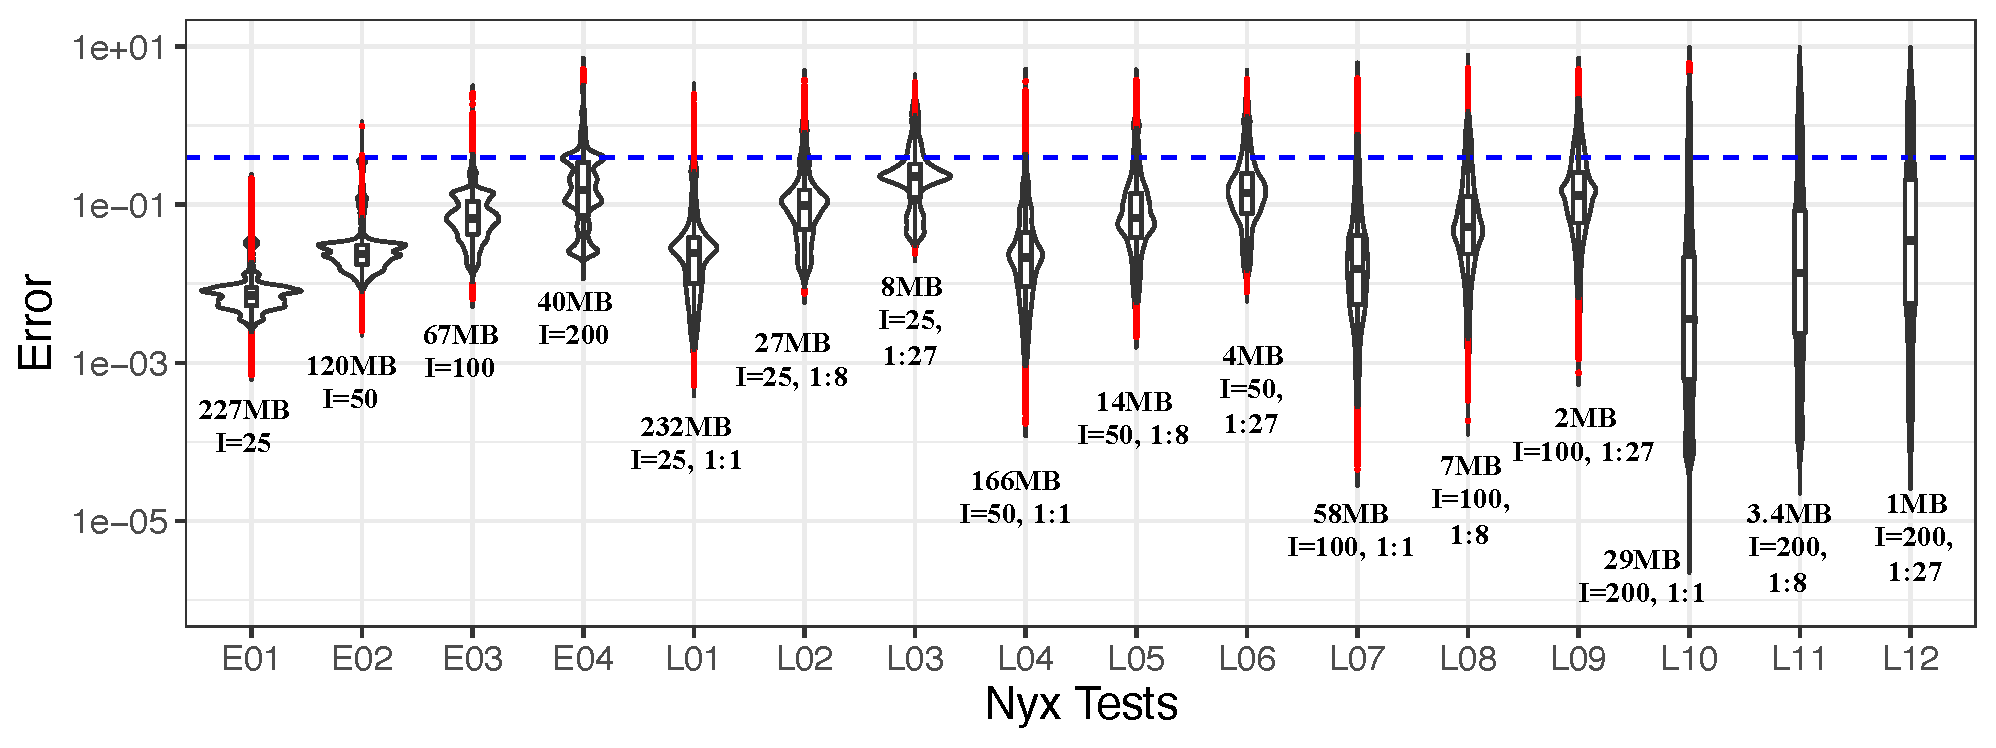
\includegraphics[width=\linewidth]{nyx_violinplot.pdf}
\vspace{-7mm}
\caption{Accuracy results for the Nyx experiments. Each violin plot shows the distribution of the particle reconstruction error for a specific configuration and the horizontal blue dashed line in the chart represents an error equivalent to a single grid cell side. The error axis uses a logarithmic scale. While Eulerian configurations contain greater uncertainty as the value of storage interval \textbf{I} increases, the Lagrangian representations offer the opportunity for improvements in accuracy. Additionally, we find high reconstruction accuracy relies on a high spatial sampling resolution as well.}
\label{fig:nyx_violinplot}
\end{figure}
\begin{figure}[!t]
\centering
\includegraphics[width=\linewidth]{nyx_figure.pdf}
\vspace{-5mm}
\caption{Pathline visualization of baryonic particles evolution in self-gravitating gas dynamics of Nyx simulation. Using 10,000 randomly seeded particles, we visualize pathlines over 300 cycles. To focus on regions where particles cluster to form dense regions, we set opacity of the pathline to be directly proportional to time. Thus, we are able to focus on clustering as well as provide context of transport toward these regions. Lagrangian representations are able to reconstruct the ground truth trajectories and capture clustering accurately when high spatial sampling is used~(1:1, 1:8). However, when using a 1:27 data reduction factor, some clusters are visualized less clearly.}
\vspace{-5mm}
\label{fig:nyx_figure}
\end{figure}
%
\noindent\textbf{Post Hoc Accuracy}
To evaluate the usefulness of Lagrangian representations to encode time-varying self-gravitating gas dynamics, we considered a $69^{3}$ grid over 400 cycles, three options for data reduction (1:1, 1:8, 1:27) and four options for \textbf{I}~(25, 50, 100, 200).
%
We constructed pathlines for 50,000 randomly placed particles during post hoc analysis.
%
We visualize the distribution of reconstruction error for all tests in Figure~\ref{fig:nyx_violinplot}.
%

The self-gravitating gas dynamics of this simulation produce a vector field that captures the transport of randomly distributed particles to multiple high-density clusters.
%
Particles travel with increasing velocity as clusters increase in density.
%
For this data, we found that Eulerian temporal subsampling performs better for small values of \textbf{I}.
%
This result can be expected given reconstruction using an Eulerian representation and fourth-order Runge Kutta interpolation remain more accurate than second-order barycentric coordinates interpolation employed to interpolate Lagrangian representations~\cite{bujack2015lagrangian}\cite{hummel2016error}.
%
However, as the value of \textbf{I} increases, the distribution of error for the Lagrangian tests indicates that a larger percentage of samples are reconstructed more accurately.
%
In particular, this is true when a high spatial sampling resolution is used.
%
Thus, particle evolution in this cosmology simulation can be tracked more accurately when a dense set of basis trajectories integrated for a long duration are interpolated.
%
In contrast, Eulerian representations become less effective at reconstructing the vector field due to increased numerical approximation.
%

We used pathlines with manually set transfer functions to visualize the evolution and clustering of particles in regions of high density.
%
The total size of the simulation vector field data used to compute the ground truth is 5.3GB.
%
We visualized a random subset of 10,000 pathlines in Figure~\ref{fig:nyx_figure} for configurations with \textbf{I} set to 25.
%
The Lagrangian representations demonstrate the ability to closely reconstruct regions where dense clusters are formed while requiring a fraction of the total simulation data size.
%
For example, the 1:8 Lagrangian configuration enables the visualization of transport to dense clusters while requiring only 27MB, i.e., a 200X data reduction of the uncompressed vector field.
%

\vspace{-3mm}
\subsection{SW4 Seismology Simulation}
\label{sec:sw4}
\noindent\textbf{In Situ Encumbrance}
For the SW4 simulation, we considered five grid sizes at varying concurrencies.
%
In each case, we used all six GPUs available on a compute node to execute the simulation and L-ISR.
%
For all L-ISR workloads tested, the execution time required per cycle remained under 0.5 seconds on average, and the maximum in situ memory required by a node was 112 MB to compute the trajectories for 4.4M particles.
%
The cost for performing L-ISR was most dependent on the number of particles and only slightly impacted by increasing grid sizes.
%
%
Referencing Figure~\ref{fig:insitucost}, although the SW4 experiments used six GPUs, we found execution time to be slower than Nyx experiments due to the use of shared memory by multiple ranks~(each has its own data block) and the high cost of launching kernels on the GPU for limited amounts of computation~(each basis particle advances by only a single step/cycle each invocation).
%
\begingroup
\setlength{\tabcolsep}{-2pt}
\begin{table*}[!ht]
\vspace{-5mm}
\begin{tabular}{|P{1.1cm}|P{1.1cm}|P{2.7cm}|P{1.3cm}|P{1.5cm}|P{1.9cm}|P{1.7cm}|P{1.7cm}|}
\hline
Nodes & Ranks & Dimensions & \textbf{Sim$_{cycle}$} & Particles & \textbf{InSituMem} & \textbf{Step} & \textbf{DAV\%} \\
\hline
\cline{1-8}
\multirow{3}{*}{1} & \multirow{3}{*}{6} & $251\times251\times70$ & 0.35s & 555k & 13.89MB & 0.0412s & 11.67\% \\
& & $335\times335\times93$  & 2.02s & 1.3M & 33.16MB & 0.2125s & 10.48\% \\
& & $501\times501\times139$  & 7.58s & 4.4M & 111.13MB & 0.3309s & 4.365\% \\ %& \multirow{13}{*}{\includegraphics[width=0.93\linewidth]{images/CPU_Step.pdf}}\\
\cline{1-3}%\cline{5-6}
\multirow{4}{*}{64} & \multirow{4}{*}{384} & \multirow{3}{*}{$1001\times1001\times276$} & 1.6s & 66k & 1.6MB & 0.0194s & 1.201\% \\
& & & 1.5s & 146k & 3.6MB & 0.0295s & 1.944\% \\
& & & 1.3s & 540k & 13.5MB & 0.0798s & 6.175\% \\
\cline{3-3}%\cline{5-6}
& & $1335\times1335\times368$ & 2.9s & 1.2M & 31.9MB & 0.2095s & 7.074\% \\
\cline{1-8}
\hline
\end{tabular}
\caption{In situ encumbrance evaluation and experiment configurations for the SW4 simulation executing on GPUs. Particles and \textbf{InSituMem} are per compute node.}
\vspace{-8mm}
\label{table:sw4_encumbrance}
\end{table*}
\endgroup

\begin{figure}[!b]
\vspace{-5mm}
\begin{subfigure}{0.495\textwidth}
\centering
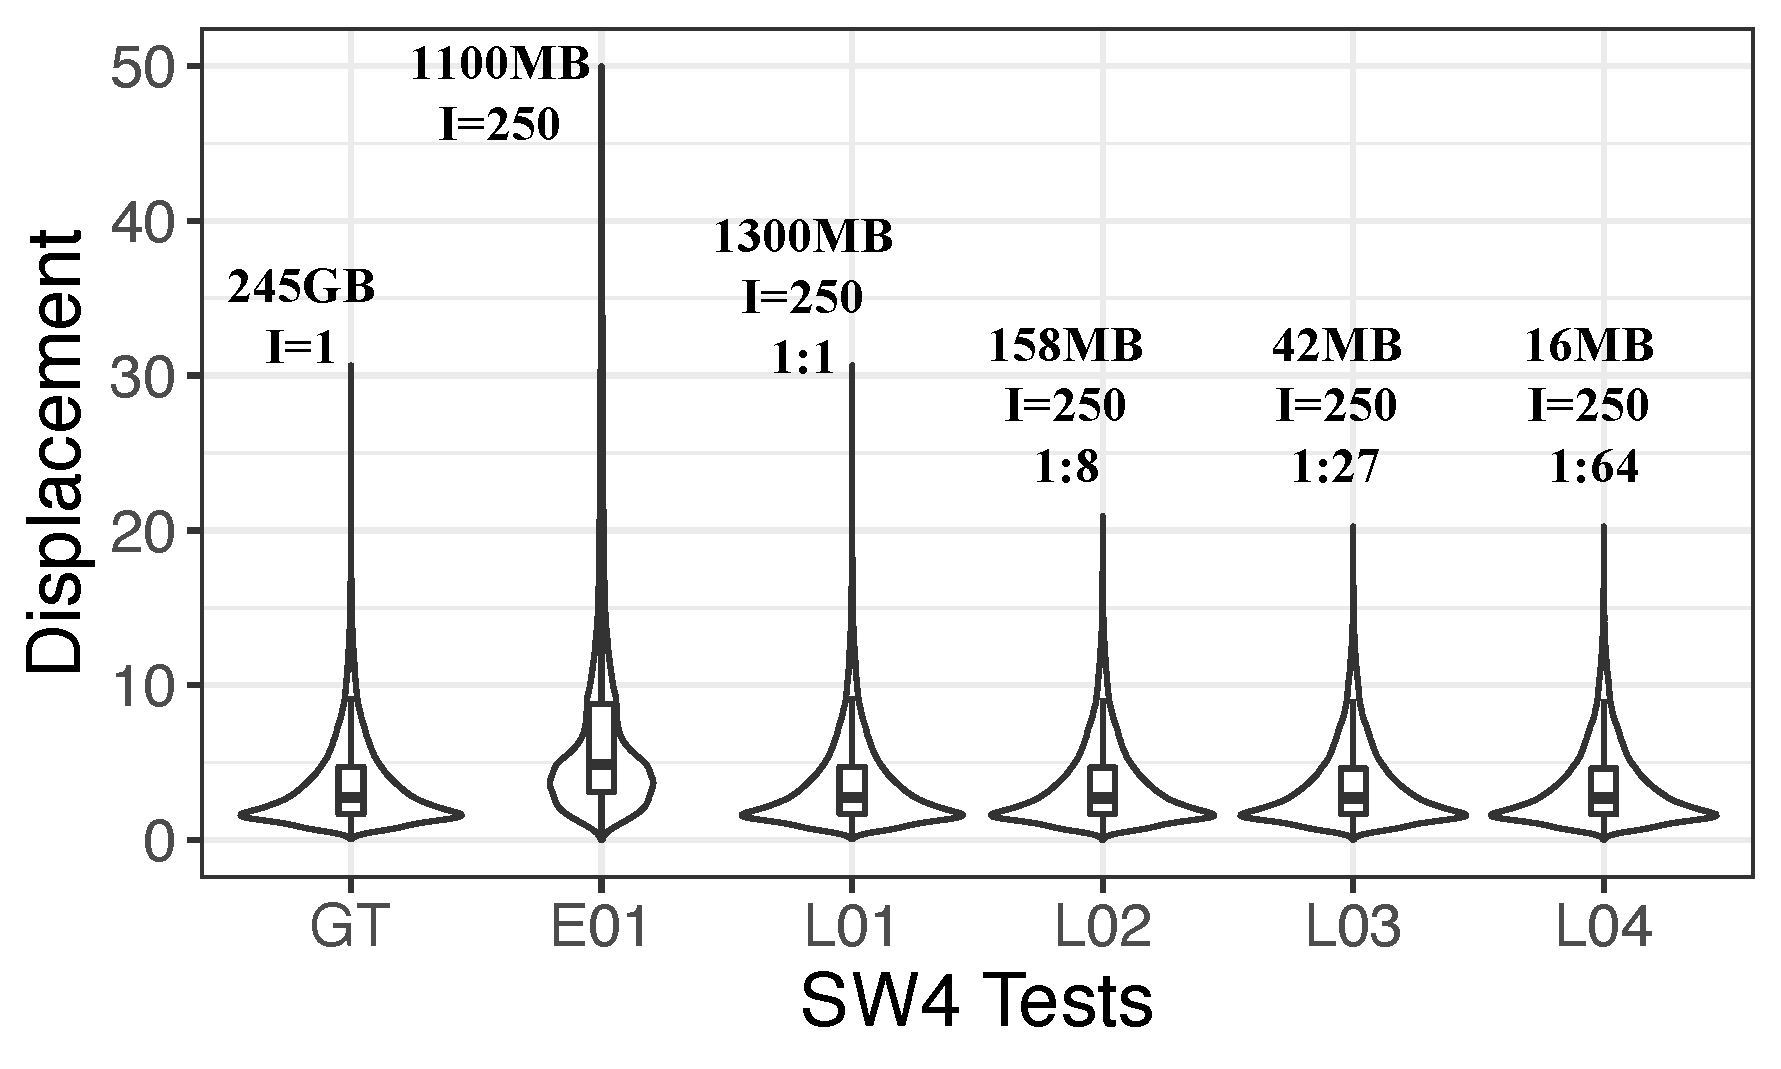
\includegraphics[width=\linewidth]{sw4_violinplot1.pdf}
\vspace{-5mm}
\caption{High displacement near the epicenter.}
\label{fig:epicenter}
\end{subfigure}
\begin{subfigure}{0.495\textwidth}
\centering
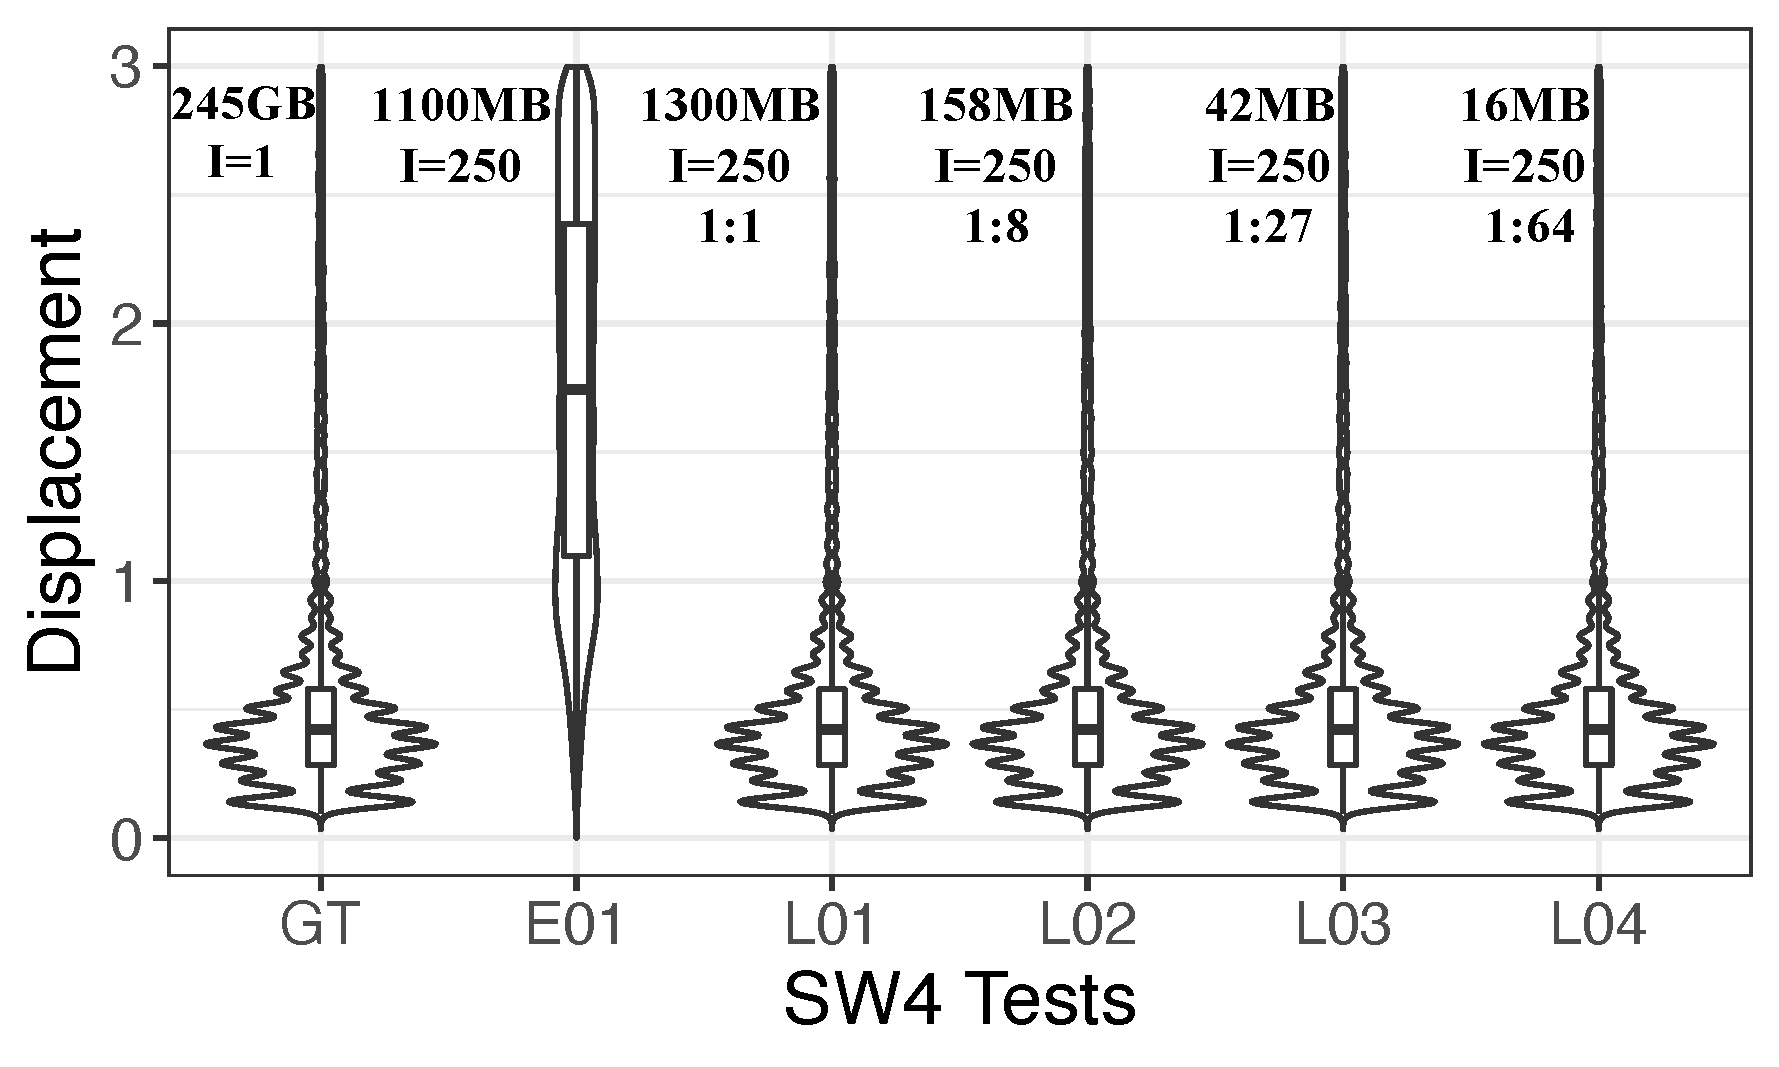
\includegraphics[width=\linewidth]{sw4_violinplot2.pdf}
\vspace{-5mm}
\caption{Low displacement away from the epicenter.}
\label{fig:clusters}
\end{subfigure}
\vspace{-2mm}
\caption{Violin plots of the distribution of particle displacement for the ground truth (GT), one Eulerian configuration and four Lagrangian configurations. The Eulerian configuration, with access to a limited number of time slices, overestimates the displacement. The Lagrangian representation captures displacement in both settings, in regions near and away from the epicenter, accurately.}
\vspace{-5mm}
\label{fig:sw4_violinplot}
\end{figure}
\begin{figure}[!t]
\centering
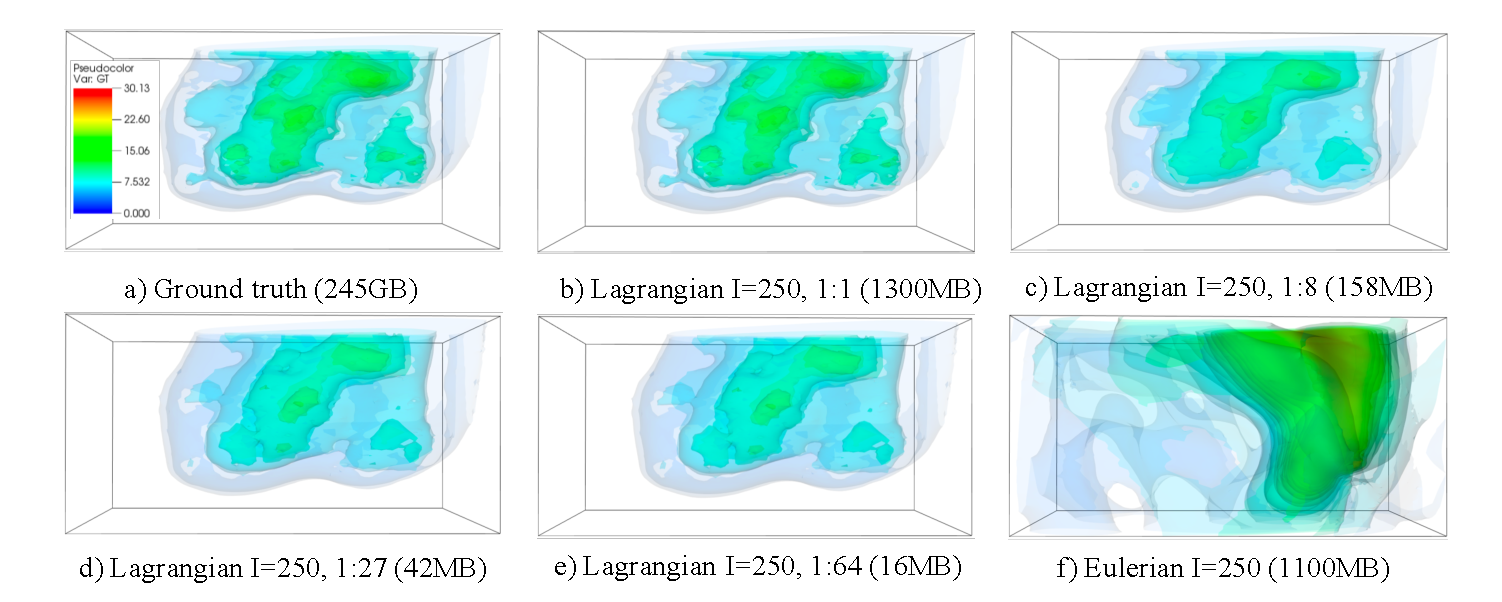
\includegraphics[width=\linewidth, trim={1cm, 0cm, 0.9cm, 0cm}, clip]{sw4_figure_small.pdf}
\vspace{-5mm}
\caption{Visualization of the displacement field derived from reduced Lagrangian representations near the epicenter using multiple isosurfaces. The ground truth is computed using 2000 cycles of the seismic wave propagation simulation. Although at higher data reduction factors regions of high displacement are underestimated, Lagrangian representations are capable of accurately reconstructing the overall feature structure.}
\vspace{-5mm}
\label{fig:sw4_figure}
\end{figure}

\noindent\textbf{Post Hoc Accuracy}
We studied the reconstruction of the time-varying displacement vector field encoding wave propagation by considering four options for data reduction~(1:1, 1:8, 1:27, 1:64) and one option for \textbf{I}~(250).
%
The ground truth was computed using data defined on a regular mesh containing 4.5M grid points over 2000 simulation cycles and required 245 GB.
%The ground truth was computed using a $381\times170\times70$ grid and 2000 simulation cycles required 245 GB.
%
The displacement was highest near the epicenter and reduced as waves propagate further away.
%
For each simulation run, we measured the displacement of 200,000 samples reconstructed near the epicenter (Figure~\ref{fig:epicenter}) and 90,000 samples reconstructed in six regions away from the epicenter (Figure~\ref{fig:clusters}).
%
Here, we directly compared against the distribution of ground truth (GT) displacement.
%
In both cases, Lagrangian representations offered significant data reduction while maintaining high accuracy.
%
We found that as the number of basis trajectories extracted reduces, the displacement for some samples near the epicenter can be underestimated.
%
In contrast, using a temporally subsampled Eulerian representation (E01) results in significant overestimation of displacement.
%
This result can be expected since temporal subsampling fails to capture the transient nature of wave propagation, whereas Lagrangian representations encoding behavior over an interval of time remain accurate.
%
Compared to Figure~\ref{fig:epicenter}, the ground truth in Figure~\ref{fig:clusters} has smaller displacement and a multimodal distribution, which is the result of samples collected from six regions of the domain away from the epicenter.
%

Figure~\ref{fig:sw4_figure} visualizes field encoding displacement over time near the epicenter using multiple semi-opaque isosurfaces.
%
Although regions of highest displacement can be underestimated as the data reduction factor increases, the overall structure is well preserved using highly compressed Lagrangian representations.
%
In all cases, Lagrangian representations required less than 1\% of the storage of the complete vector data.

\vspace{-2mm}
\section{Conclusion}
\label{sec:conclusion}
Accurate exploratory analysis and visualization of time-varying vector fields is challenging.
% 
On the one hand, it can be performed accurately if the entire spatiotemporal resolution is available.
%
However, storing all the data to disk for exploratory post hoc analysis is expensive.
%
On the other hand, if subsets of the data are stored, predicting uncertainty and variability of accuracy for analysis techniques post hoc is difficult.
%
In this context, Lagrangian representations computed using the full spatiotemporal resolution via in situ processing demonstrate the potential to enable accurate exploratory time-varying vector field analysis for reduced data storage costs.


%can enable exploratory time-varying vector field analysis.

For wider adoption and consideration of Lagrangian representations, an important step is characterization of effectiveness across a broad range of real-world applications.
%
In this paper, we investigated in situ reduction via Lagrangian representations for vector fields from Nyx cosmology and SW4 seismology simulations.
%
For the Nyx cosmology simulation, we found that Lagrangian representations are sensitive to both the spatial and temporal sampling rate, notably providing higher reconstruction accuracy when basis trajectories are computed using a high spatial and low temporal resolution.
%
For the SW4 seismology simulation, we found Lagrangian representations are well suited to capture the transient seismic waves and offer high data reduction options for a small loss of accuracy.
%
For both simulations, the percentage of execution time spent on computing the Lagrangian representation in situ was under 10\% in most cases.
%
Overall, we believe the findings of this study demonstrates that two computational science simulations considered benefit from Lagrangian representations for time-varying vector field exploration.
%
This finding also provides confidence that more computational areas can benefit, and we encourage future work in this direction.

\vspace{-2mm}
\section*{Acknowledgment}
This research was supported by the Exascale Computing Project~(17-SC-20-SC), a collaborative effort of the U.S. Department of Energy Office of Science and the National Nuclear Security Administration. 
%
%This research used resources of the Oak Ridge Leadership Computing Facility at the Oak Ridge National Laboratory, which is supported by the Office of Science of the U.S. Department of Energy under Contract No. DE-AC05-00OR22725.
%
This research used resources of the Oak Ridge Leadership Computing Facility at the Oak Ridge National Laboratory, which is supported by the Office of Science of the U.S. Department of Energy under Contract No. DE-AC05-00OR22725.
%

\bibliographystyle{splncs04}
\bibliography{sane_iccs21}
\end{document}
